\chapter{\label{chap:implementierung}WIP Implementierung der Prototypen}
In diesem Kaptitel wird nach dem in Kapitel \ref{chap:konzeption} präsentiertem Lösungsweg die detaillierte Beschreibung der technischen Realisierung der Prototypen vorgestellt.\\
\todo{Nach der Beschreibung der Hauptkomponente wird auf die Umsetzung der Offlinefunktionalität und des Konfliktmanagements eingegangen. Im Zuge dessen wird ... vorgestellt...}
%
%
%
\section{WIP Hauptmodul Contacts}

Kontakte lesen, anlegen, bearbeiten, löschen
Couch ermittelt Delta über die Revisionsnummer und sendet nur die neuen Daten.
CRUD, toggleEdit, getConflictRevisions, chooseRev()\\
Redux: Contacts= ContactsView, ContactsContainer, reducer/actions
%
%
%
\section{WIP Offlinefunktionalität}
Die Prototypen \it{amilia-qouch} und \it{amilia-rdx} sind vollständig offline verwendbar.
%Das heißt, dass nach einem initialen Besuch der Webseite ​https://kamrat.xyz diese Seite auch ohne eine Internetverbindung angesteuert werden kann.
Alle in \autoref{chap:offlinefirst} beschriebenen Grundvoraussetzungen werden von beiden Prototypen erfüllt und sämtliche umgesetzten Funktionen sind sowohl mit als auch ohne Internetverbindung durchführbar.
%
%
\sub{Datenspeicherung}
Cachen der Assets geht erst nach den build -> ServiceWorker\\
BenutzerInnengenerierte Daten:
Screenshots!\\
Redux Offline: LocalStorage\\
PouchDB: IndexedDB
%
%
\sub{Datenbanksynchronisation}
Redux: discard überchreiben weil ROLLBACK nicht immer retried, obwohl das so in der Dokumentation steht.
Wie wurde CRUD implementiert?\\
%
%
%
\section{WIP Konfliktmanagement}
Wie kann ein Konflikt erzeugt werden?\\
(manuell -- siehe \ref{sub:detect})
Modal:
\begin{figure}[H]
  \centering
  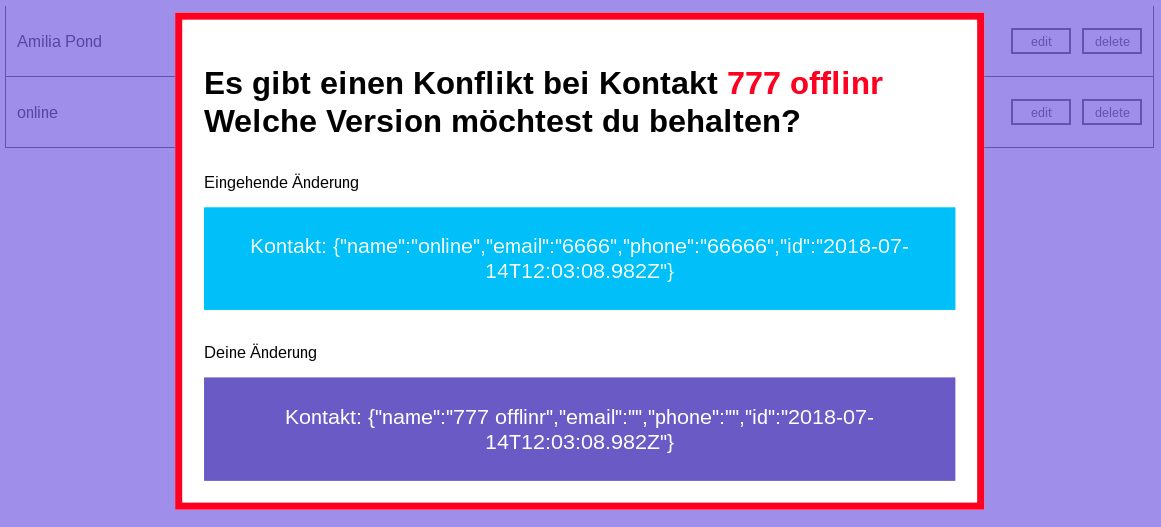
\includegraphics[width=\textwidth]{impl/Modal}
  \grayRule
  \caption{Konfliktdialog in Aktion}
  \label{fig:modal}
\end{figure}
Modal ist nicht bei Redux offline enthalten, das es nicht die Möglichkeit bietet Konflikte zu erkennen, gescheige denn zu speichern.
%
%
%
%
% Installationsanleitung
%
\section{WIP Installationsanleitung}
\todo{build und so}
Beide entwickelten Prototypen sind als öffentliche Repositories auf GitHub\footnote{Software--Entwicklungs--Plattform \url{https://github.com/}} zu finden. 
Um sie zu installieren müssen folgende Schritte ausgeführt werden.
\sub{amilia-qouch}
1. Zuerst muss das Repository kopiert werden:
\lstset{language=sh, caption={},belowcaptionskip=0.3\baselineskip}
\begin{lstlisting}
git clone git@github.com:hulkoba/amilia-qouch.git
# oder
git clone https://github.com/hulkoba/amilia-qouch.git
\end{lstlisting}
2. Dann muss man in das Verzeichnis navigieren und alle Abhängigkeiten installieren.
\begin{lstlisting}
cd amilia-qouch
npm install
\end{lstlisting}
3. Mittels
\begin{lstlisting}
npm start
\end{lstlisting}
wird die Anwendung gestartet.
%
\sub{amilia-rdx}
1. Auch hier muss das Repository zuerst kopiert werden:
\lstset{language=sh, caption={},belowcaptionskip=0.3\baselineskip}
\begin{lstlisting}
git clone git@github.com:hulkoba/amilia-rdx.git
# oder
git clone https://github.com/hulkoba/amilia-rdx.git
\end{lstlisting}
2. Schritt zwei ist identisch mit dem in der \tt{amilia-qouch} Anleitung\\
3. Mittels
\begin{lstlisting}
npm run server
npm start
\end{lstlisting}
wird zuerst der Server, dann die Anwendung gestartet.

%
% Testfälle
%
\section{\label{chap:impl:test}Testfälle}
\section{\label{sec:impl:test}Testfälle}
Folgende Testfälle zur Offlinefunktionalität werden während der Entwicklung stetig durchgeführt. Das erfolgreiche Bestehen dieser Tests ist eine notwendige Qualitätseigenschaft der zu entwickelnden Prototypen.
\begin{description}[leftmargin=0.7cm,style=nextline]
\item[Netzwerkstatus:] 
Die Anwendung muss zu jeder Zeit den korrekten Netzwerkstatus anzeigen.\\
\item[Kontakte lesen:] 
Die Anwendung bei jedem Start die Kontakte aus dem lokalen Speicher oder aus der \it{Datenbank} laden.\\
\item[Kontakt anlegen:] 
Die Anwendung muss zu jedem Zeitpunkt in der Lage sein einen Kontakt mit jedem seiner Attribute anzulegen. Dazu muss er immer lokal gespeichert werden und sobald eine Internetverbindung besteht, persistiert werden.
Das Anlegen eines Kontakts im Offlinestatus ist für die Konfliktforcierung erforderlich.\\
\item[Kontakt bearbeiten:] 
Die Anwendung muss zu jedem Zeitpunkt in der Lage sein einen Kontakt mit jedem seiner Attribute zu bearbeiten. Ist keine Internetverbindung vorhanden, müssen die Änderungen lokal übernommen und später, sobald sich der Netzwerkstatus ändert, synchronisiert werden.
Das Bearbeiten eines Kontakts im Offlinestatus ist für die Konfliktforcierung erforderlich.\\
\item[Kontakt löschen:] 
Die Anwendung muss zu jedem Zeitpunkt in der Lage sein einen Kontakt zu löschen.
Das Löschen eines Kontakts im Offlinestatus ist für die Konfliktforcierung erforderlich.
\end{description}